\subsection{Моделирование тепловых процессов, протекающих в электронном модуле и устройстве в целом}

Результаты теплового анализа для первого варианта компоновки ПП
в \textit{SOLIDWORKS Simulation} представлены на рисунке 14.

\begin{figure}[h]
  \centering
  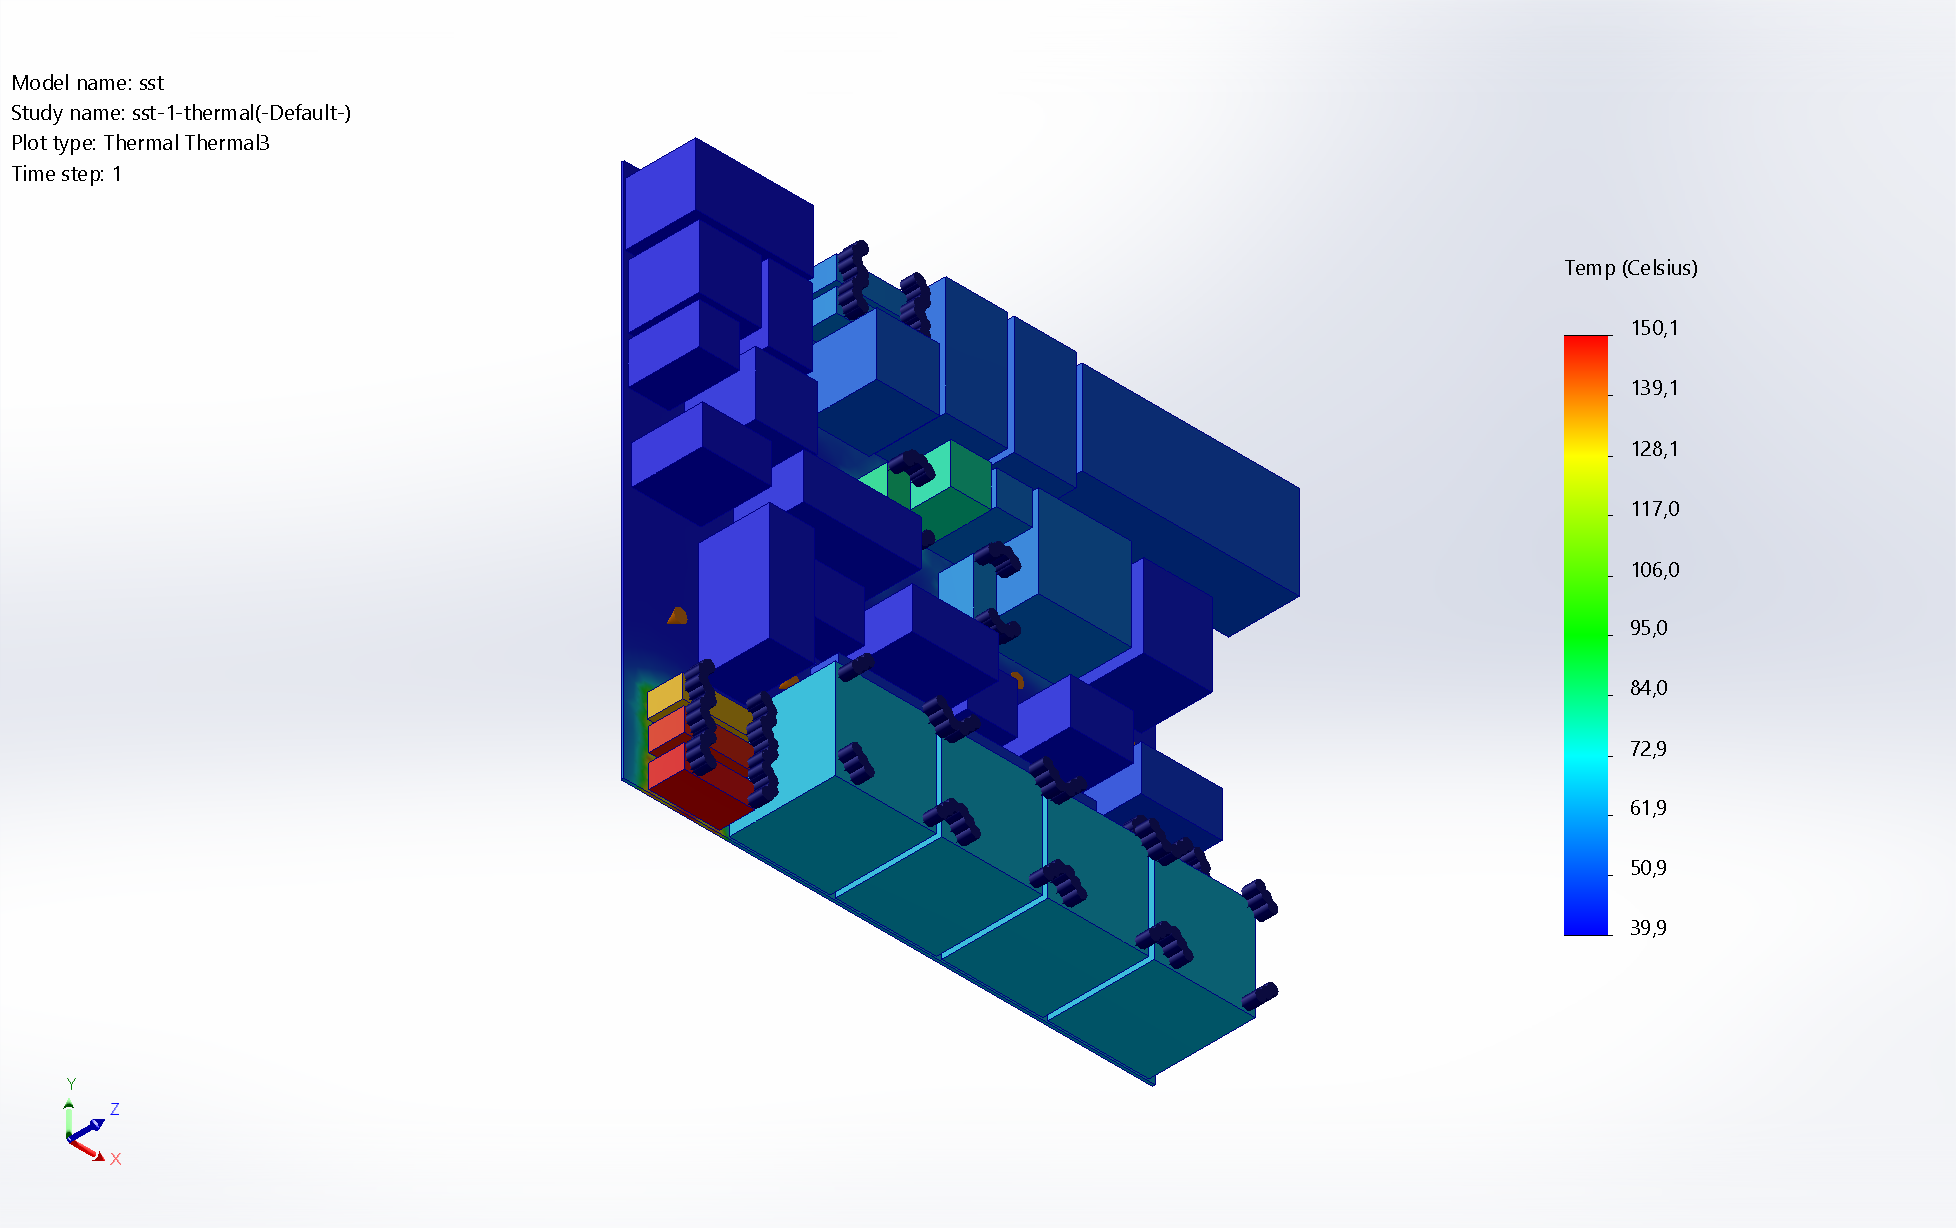
\includegraphics[scale=0.3]{../img/sst-1/thermal/top_view.png}
  \caption{Результаты теплового анализа в \textit{SOLIDWORKS Simulation}
    для первого варианта компоновки}
\end{figure}

Результаты теплового анализа для второго варианта компоновки ПП в
\textit{SOLIDWORKS Simulation} представлены на рисунке 15.

\begin{figure}[h]
  \centering
  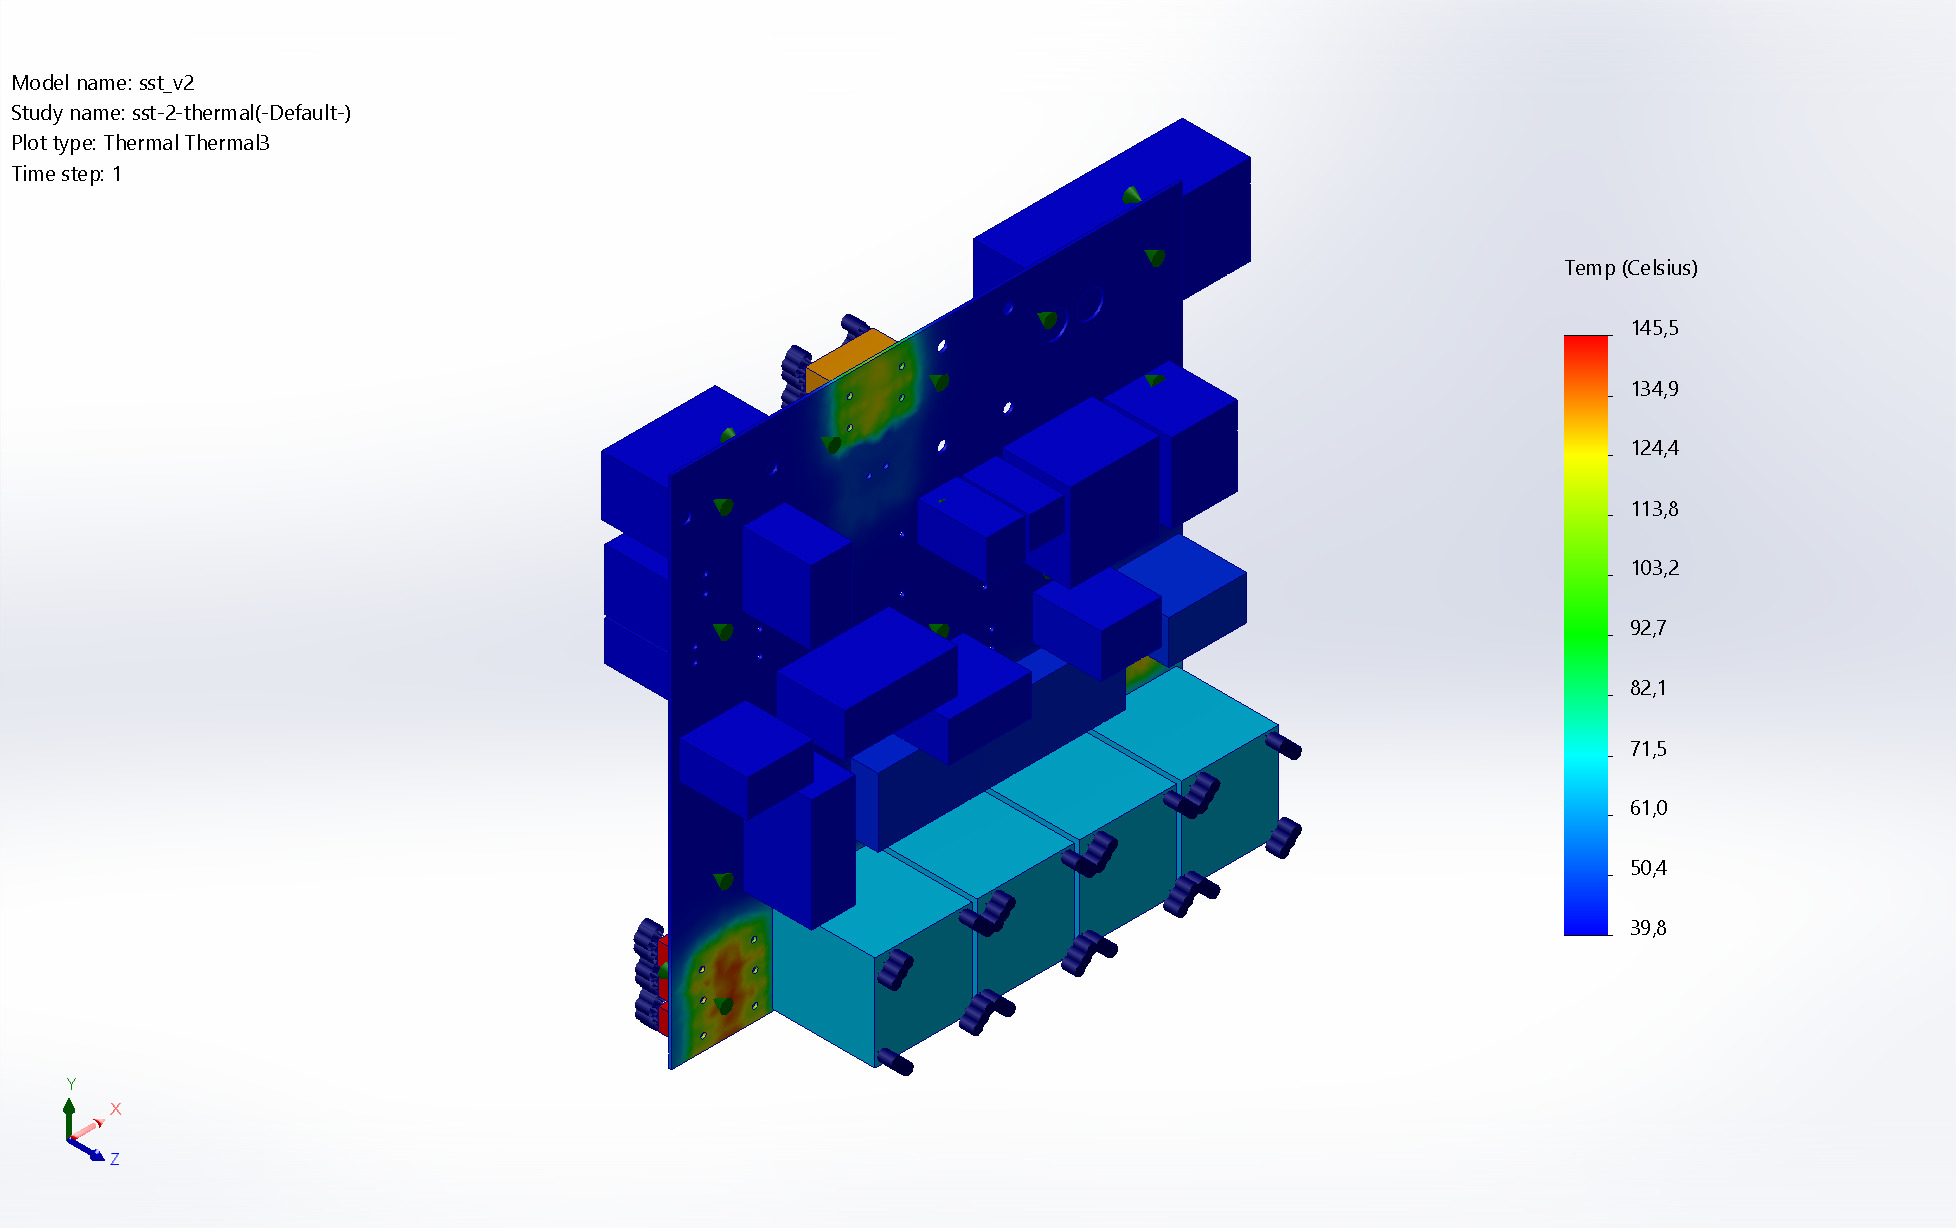
\includegraphics[scale=0.3]{../img/sst-2/thermal/sst_v2-sst-2-thermal-Thermal-Thermal3.jpg}
  \caption{Результаты теплового аналиаза в \textit{SOLIDWORKS Simulation}
    для второго варианта компновки}
\end{figure}

Результаты теплового анализа для третьего варианта компоновки ПП в
\textit{SOLIDWORKS Simulation} представлены на рисунке 16.
\begin{figure}[h]
  \centering
  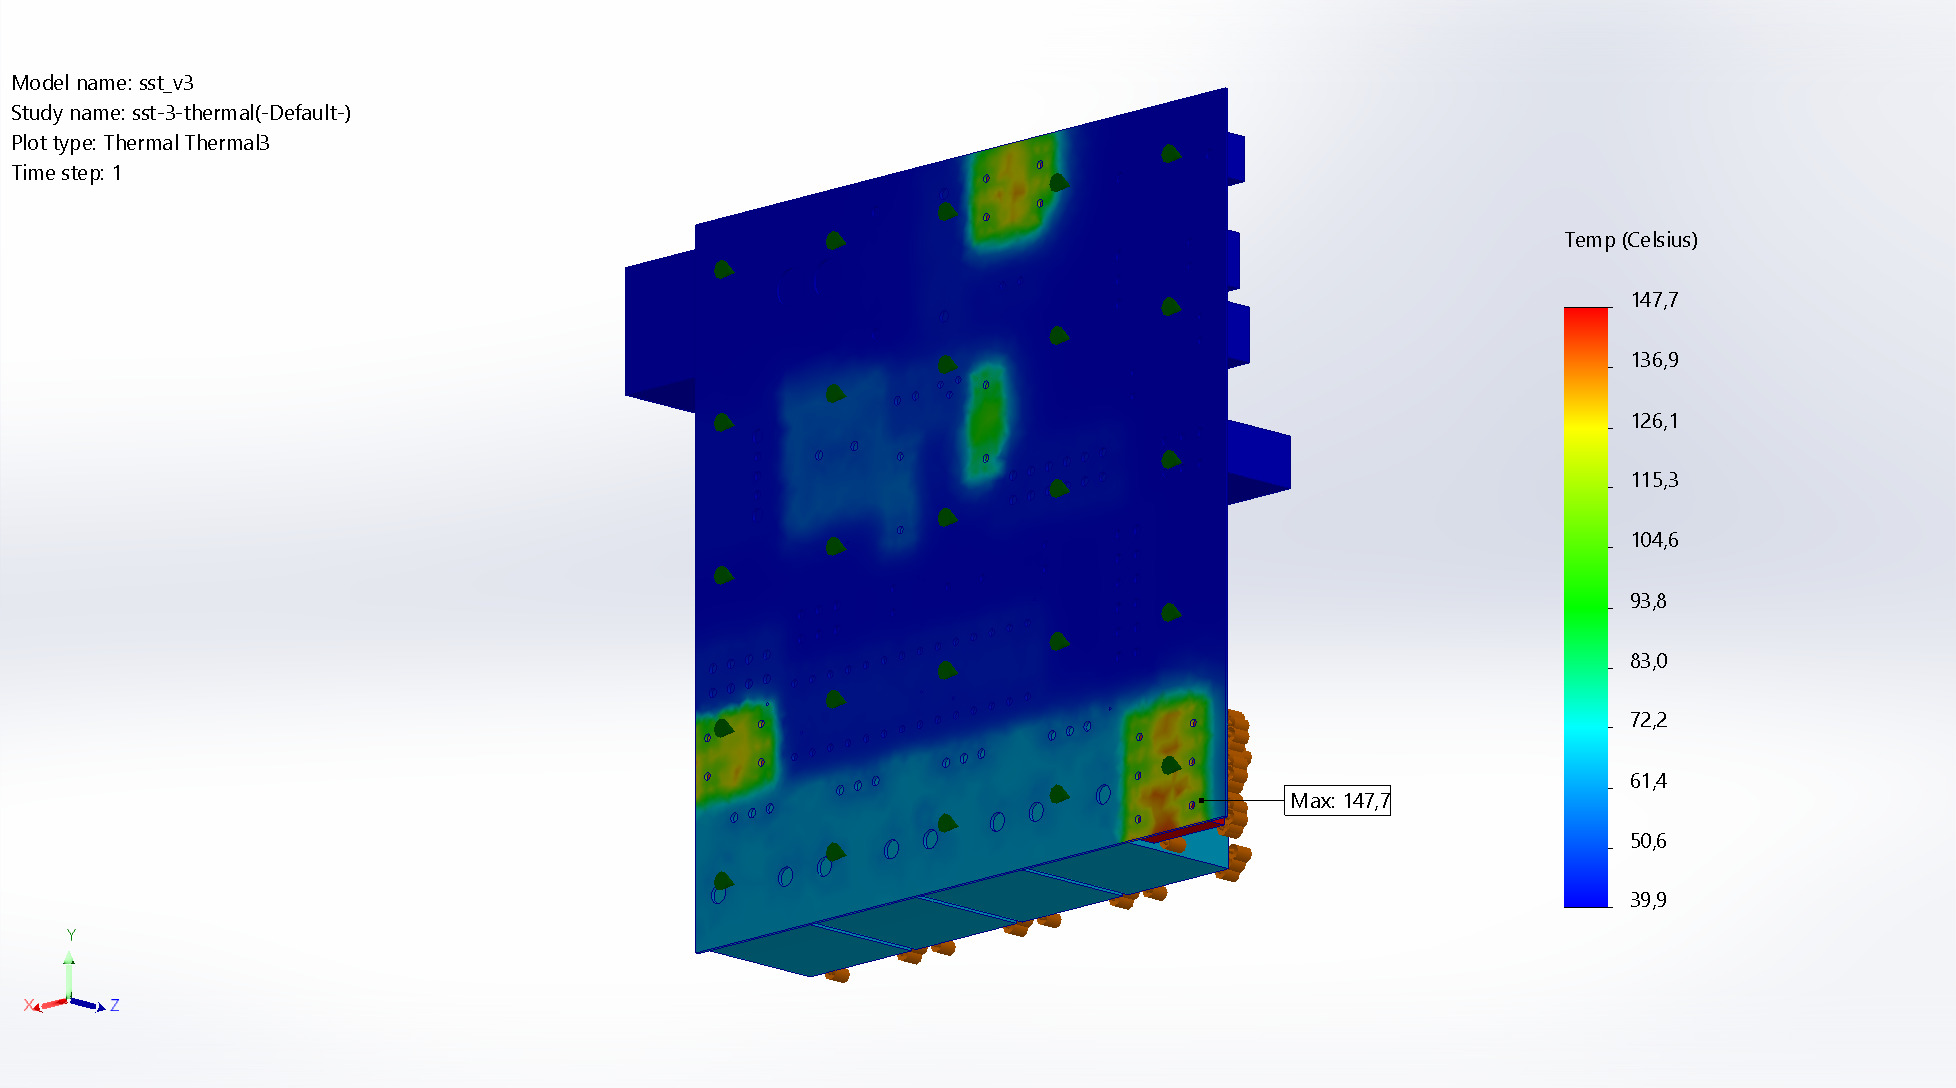
\includegraphics[scale=0.3]{../img/sst-3/thermal/sst_v3-sst-3-thermal-Thermal-Thermal3.jpg}
  \caption{Результаты теплового аналиаза в \textit{SOLIDWORKS Simulation}
    для второго варианта компновки}
\end{figure}

Результаты тепловго анализа для первого варианта компоновки ПП в
\textit{COMSOL Multiphysics} представлены на рисунке 17.
\begin{figure}[h]
  \centering
  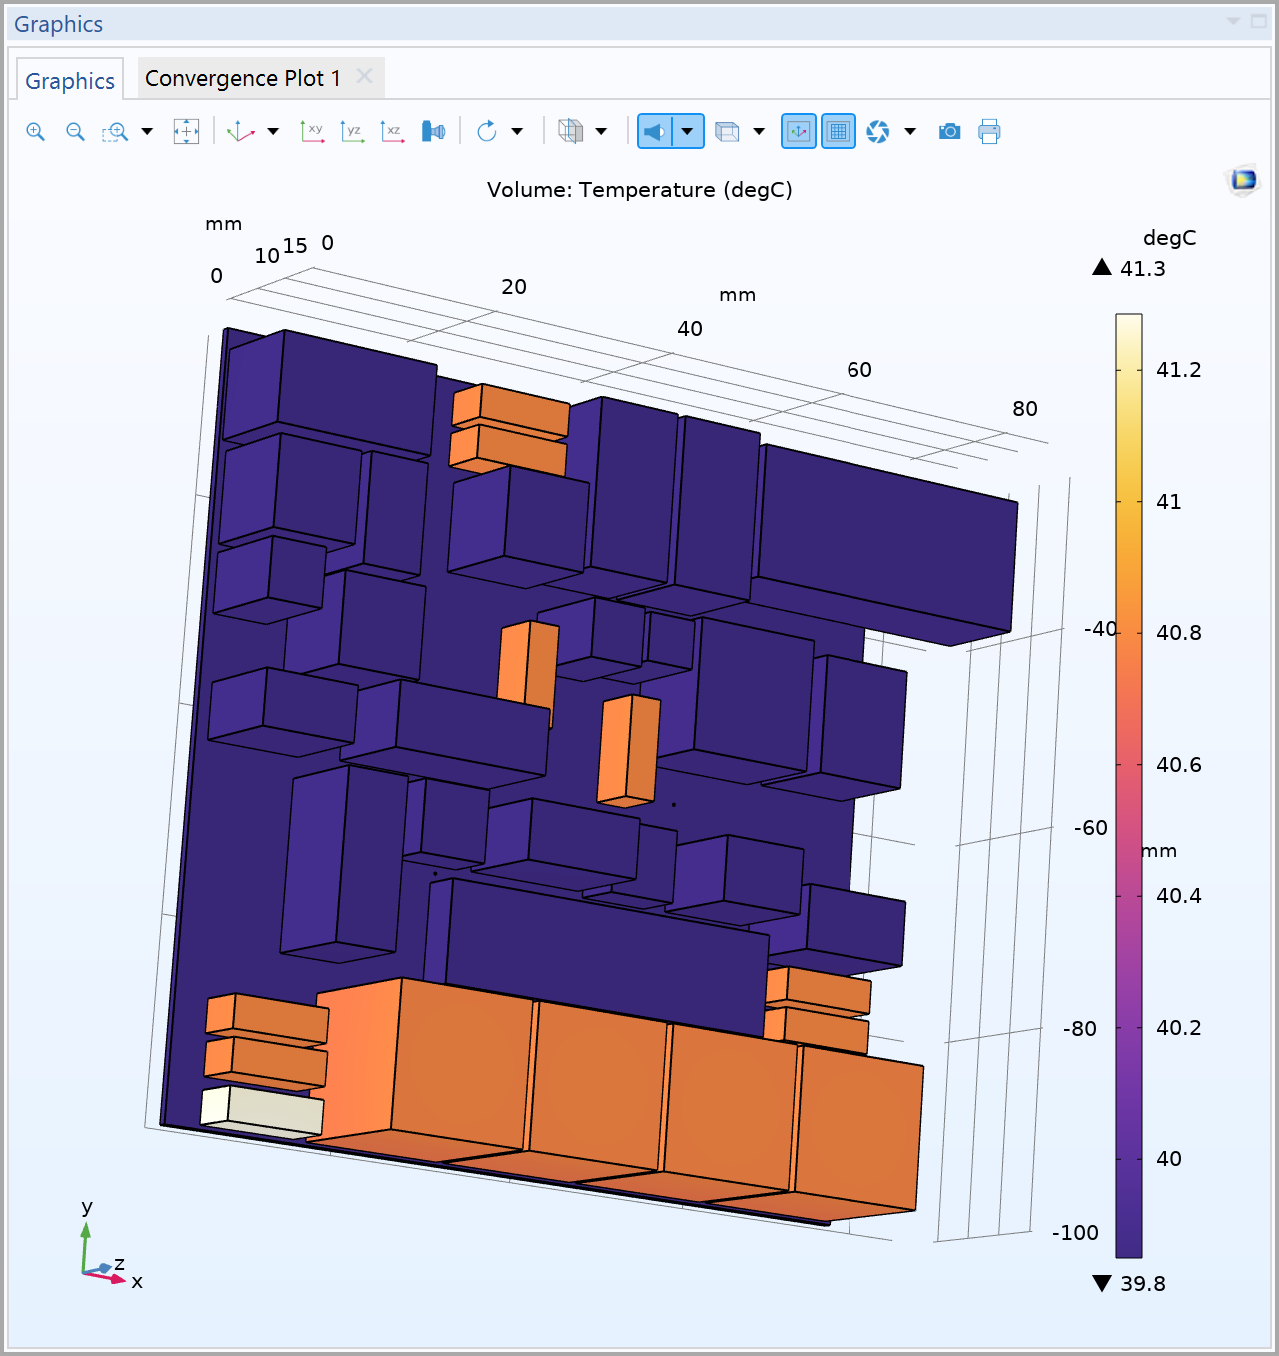
\includegraphics[scale=0.5]{../img/scrot/Screenshot-2024-05-16-022638.png}
  \caption{Результаты теплового анализа в \textit{COMSOL Multhiphysics}
    для первого варианта компоновки}
\end{figure}

Результаты теплвого анализа для второго варианта компоновки ПП в
\textit{COMSOL Multiphysics} представлены на рисунке 18.

\begin{figure}[h]
  \centering
  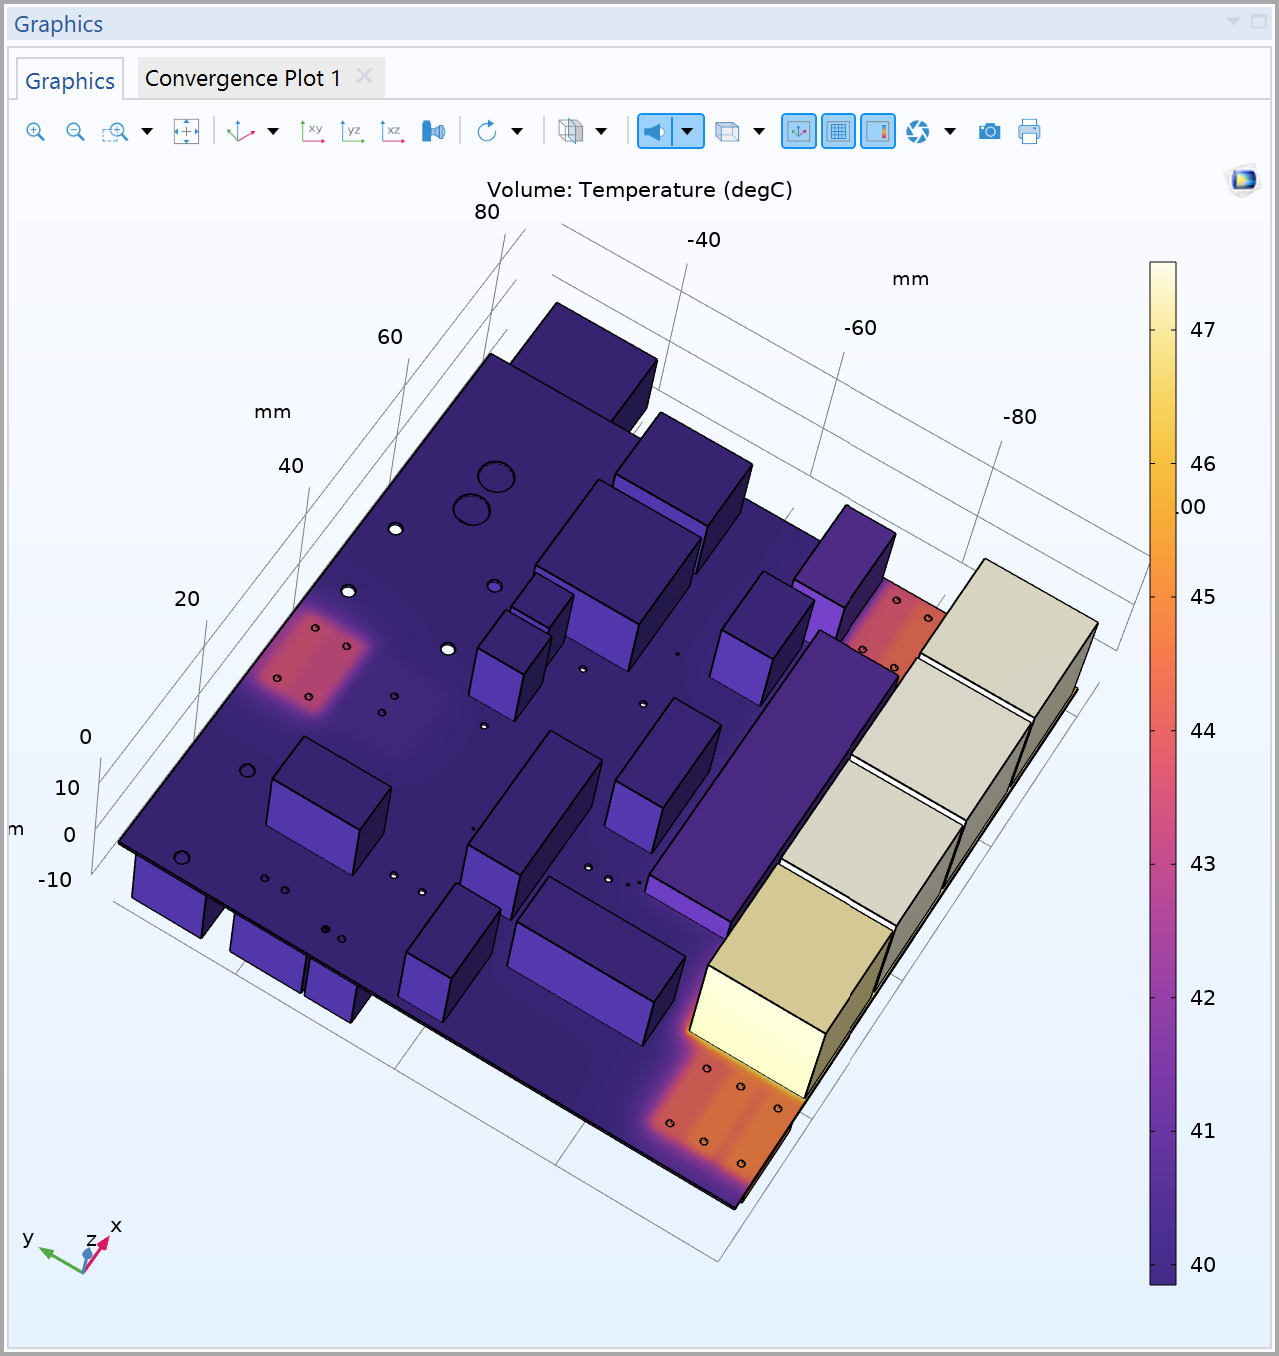
\includegraphics[scale=0.5]{../img/scrot/Screenshot-2024-05-16-023133.png}
  \caption{Результаты теплвого анализа в \textit{COMSOL Multiphysics}
  для второго варианта компоновки}

\end{figure}

Результаты тепловго анализа для третьего варианта комопновки ПП в
\textit{COMSOL Multiphysics} представлены на рисунке 19.
\begin{figure}[H]
  \centering
  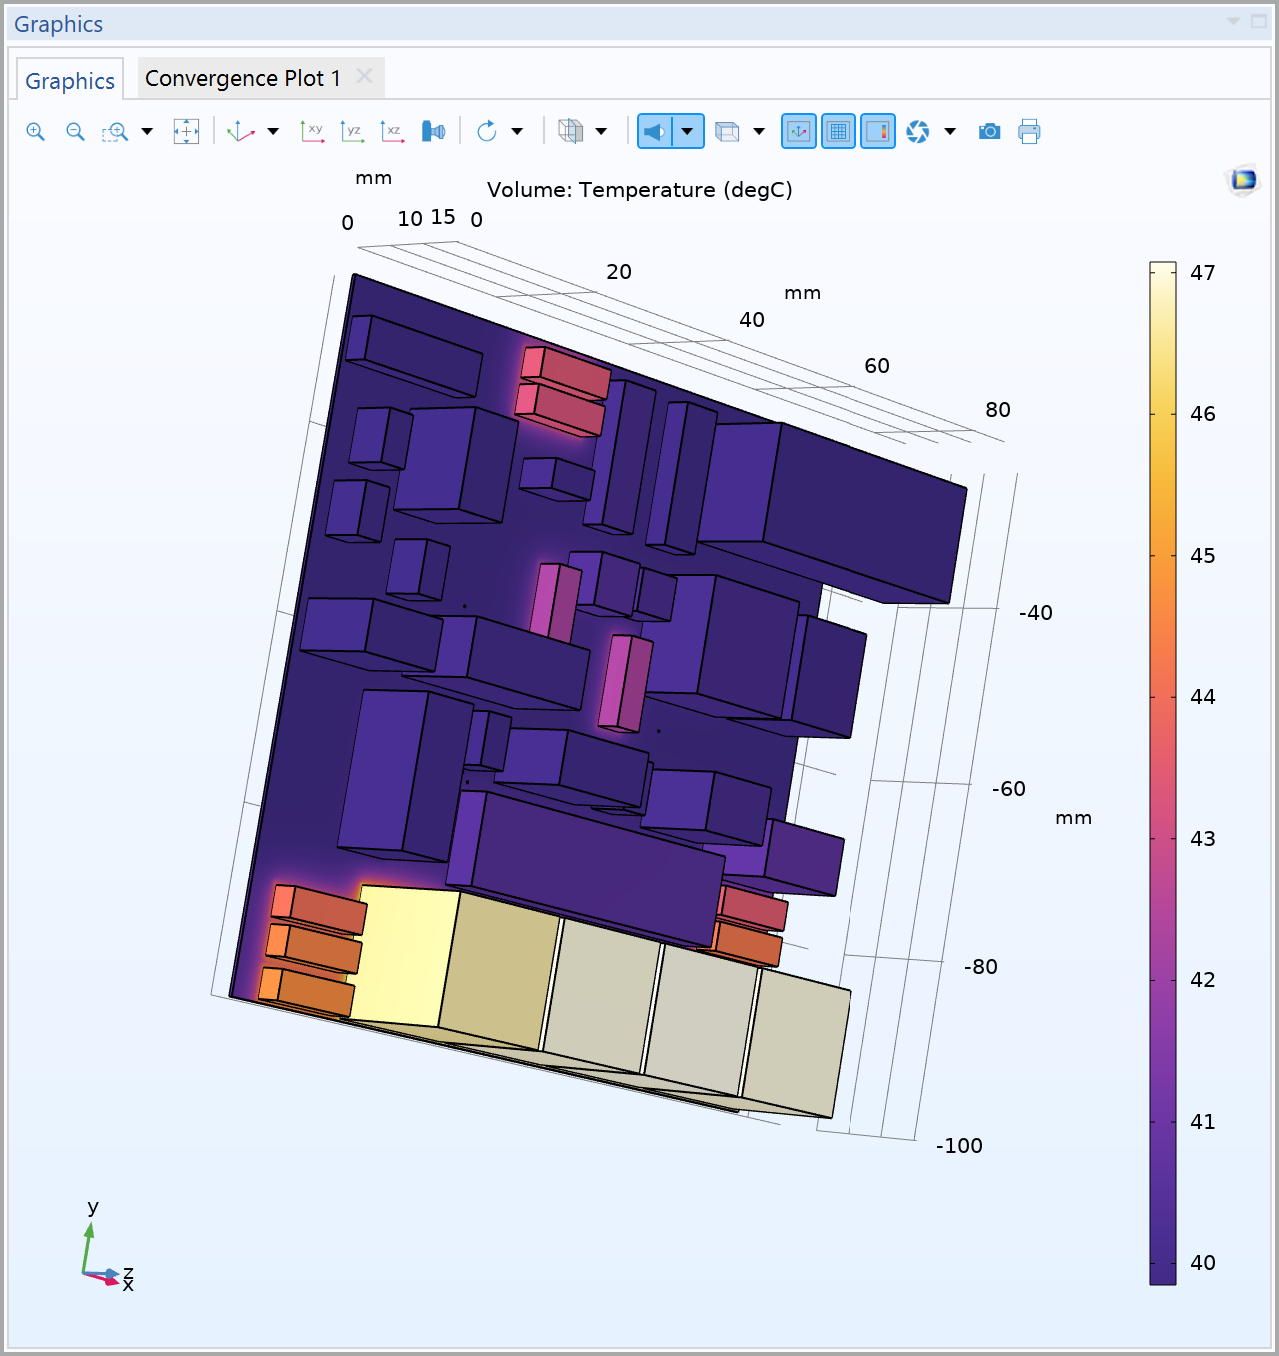
\includegraphics[scale=0.5]{../img/scrot/Screenshot-2024-05-16-024105.png}
  \caption{Результаты теплвого анализа в \textit{COMSOL Multiphysics}
  для третьего варианта компоновки}

\end{figure}

